\documentclass[10pt,letterpaper]{article}
\usepackage[
    letterpaper,
    top=0.65in,
    bottom=0.65in,
    left=0.7in,
    right=0.7in,
    headheight=14pt,
    footskip=18pt
]{geometry}

\usepackage[utf8]{inputenc}
\usepackage[T1]{fontenc}
\usepackage{lmodern}
\usepackage{microtype}
\usepackage{graphicx}
\usepackage{booktabs}
\usepackage{tabularx}
\usepackage{xcolor}
\usepackage{fancyhdr}
\usepackage{titlesec}
\usepackage{enumitem}
\usepackage{caption}
\usepackage{tcolorbox}
\usepackage{needspace}
\usepackage[
    colorlinks=true,
    linkcolor=cobalt,
    urlcolor=cobalt,
    citecolor=cobalt,
    pdfauthor={Steve Blanding / The Pack Rat Preservation Project},
    pdftitle={The Pack Rat (1992) — Definitive Player Guide and Cheat Sheet}
]{hyperref}

% Academic Color Palette (Nordic Deep & Retro Gold)
\definecolor{cobalt}{RGB}{20, 55, 125}
\definecolor{teal}{RGB}{12, 115, 135}
\definecolor{crimson}{RGB}{185, 28, 48}
\definecolor{gold}{RGB}{180, 120, 15}
\definecolor{slatebg}{RGB}{247, 249, 252}
\definecolor{cardbg}{RGB}{252, 253, 255}
\definecolor{borderline}{RGB}{205, 218, 232}
\definecolor{charcoal}{RGB}{35, 40, 50}

\color{charcoal}

% Page Header/Footer
\pagestyle{fancy}
\fancyhf{}
\lhead{\textsc{\small\textcolor{cobalt}{The Pack Rat (1992) — Definitive Walkthrough \& Cheat Guide}}}
\rhead{\textsc{\small\textcolor{gray}{Preservation Edition}}}
\cfoot{\thepage}
\renewcommand{\headrulewidth}{0.5pt}
\renewcommand{\footrulewidth}{0pt}

% Section Titles Styling
\titleformat{\section}{\color{cobalt}\normalfont\Large\bfseries\scshape}{\thesection.}{0.7em}{}[\titlerule]
\titleformat{\subsection}{\color{teal}\normalfont\large\bfseries}{\thesubsection}{0.5em}{}
\titleformat{\subsubsection}{\color{charcoal}\normalfont\normalsize\bfseries}{\thesubsubsection}{0.4em}{}

\titlespacing*{\section}{0pt}{8pt}{4pt}
\titlespacing*{\subsection}{0pt}{6pt}{3pt}

% Custom Styled Secret Cards
\newtcolorbox{secretcard}[2][cobalt]{
    colback=cardbg,
    colframe=#1,
    coltitle=white,
    title=\textbf{#2},
    fonttitle=\bfseries\small,
    sharp corners=south,
    rounded corners=north,
    boxrule=1pt,
    arc=3pt,
    top=5pt, bottom=5pt, left=6pt, right=6pt,
    before skip=6pt, after skip=6pt
}

\newtcolorbox{tipbox}[1]{
    colback=slatebg,
    colframe=gold,
    coltitle=white,
    title=\textbf{#1},
    fonttitle=\bfseries\small,
    sharp corners=south,
    rounded corners=north,
    boxrule=1pt,
    arc=3pt,
    top=4pt, bottom=4pt, left=8pt, right=8pt,
    before skip=4pt, after skip=4pt
}

\begin{document}

% Title Block
\begin{center}
    {\Huge\textbf{\textsc{\textcolor{cobalt}{The Pack Rat}}}}\\[2pt]
    {\large\textbf{\textsc{\textcolor{gold}{Definitive Player Walkthrough \& Secret Cheat Guide}}}}\\[3pt]
    {\small Author: Authentic 1992 Preservation Team \quad\textbullet\quad Platform: PC / Web Retro Revival \quad\textbullet\quad 16 Levels Complete}\\[5pt]
    \rule{\linewidth}{1.2pt}
\end{center}

\vspace{-0.7em}

\section{Introduction: The Labyrinth Beyond the Living Room}
In 1992, Steve Blanding released \emph{The Pack Rat}, a deceptively deep puzzle-platformer. On its surface, the game seems like a straightforward obstacle course where a clever rodent scampers past snapping mousetraps, coils around thread spools, and slides ice blocks to collect cheese. 

However, hidden beneath the floorboards lies an intricate, branching network of \textbf{16 interconnected stages}:
\begin{itemize}[noitemsep,topsep=1pt]
    \item \textbf{10 Main Campaign Levels (Levels 1--10)}: The primary house gauntlet leading from the lower foundations up through the perilous attic and kitchen.
    \item \textbf{5 Secret Bonus Levels (Levels 11--15)}: Elusive subterranean chambers packed with bonus cheese, coins, and warp passages that bypass treacherous gauntlets.
    \item \textbf{1 Grand Finale (Level 16)}: The ultimate high-voltage laboratory where the true ending awaits.
\end{itemize}

\begin{tipbox}{The Golden Rule of The Pack Rat}
The original 1992 game manual teased: \emph{“Not everything is what it seems. Some things on the screen are illusionary. You can walk right through illusionary bricks and you will not be killed by illusionary water.”} This guide reveals every false wall, harmless pool, and decoy trap with human landmarks and clear visual routes.
\end{tipbox}

\vspace{-0.2em}

\section{Master Level Progression Flowchart}
Unlike traditional linear platformers, \emph{The Pack Rat} branches dramatically. Reaching the true ending requires choosing the right mouse holes and avoiding deceptive loops that dump you back at the beginning of the house!

\begin{center}
    \fboxsep=0pt\fboxrule=0.8pt\fcolorbox{borderline}{white}{%
        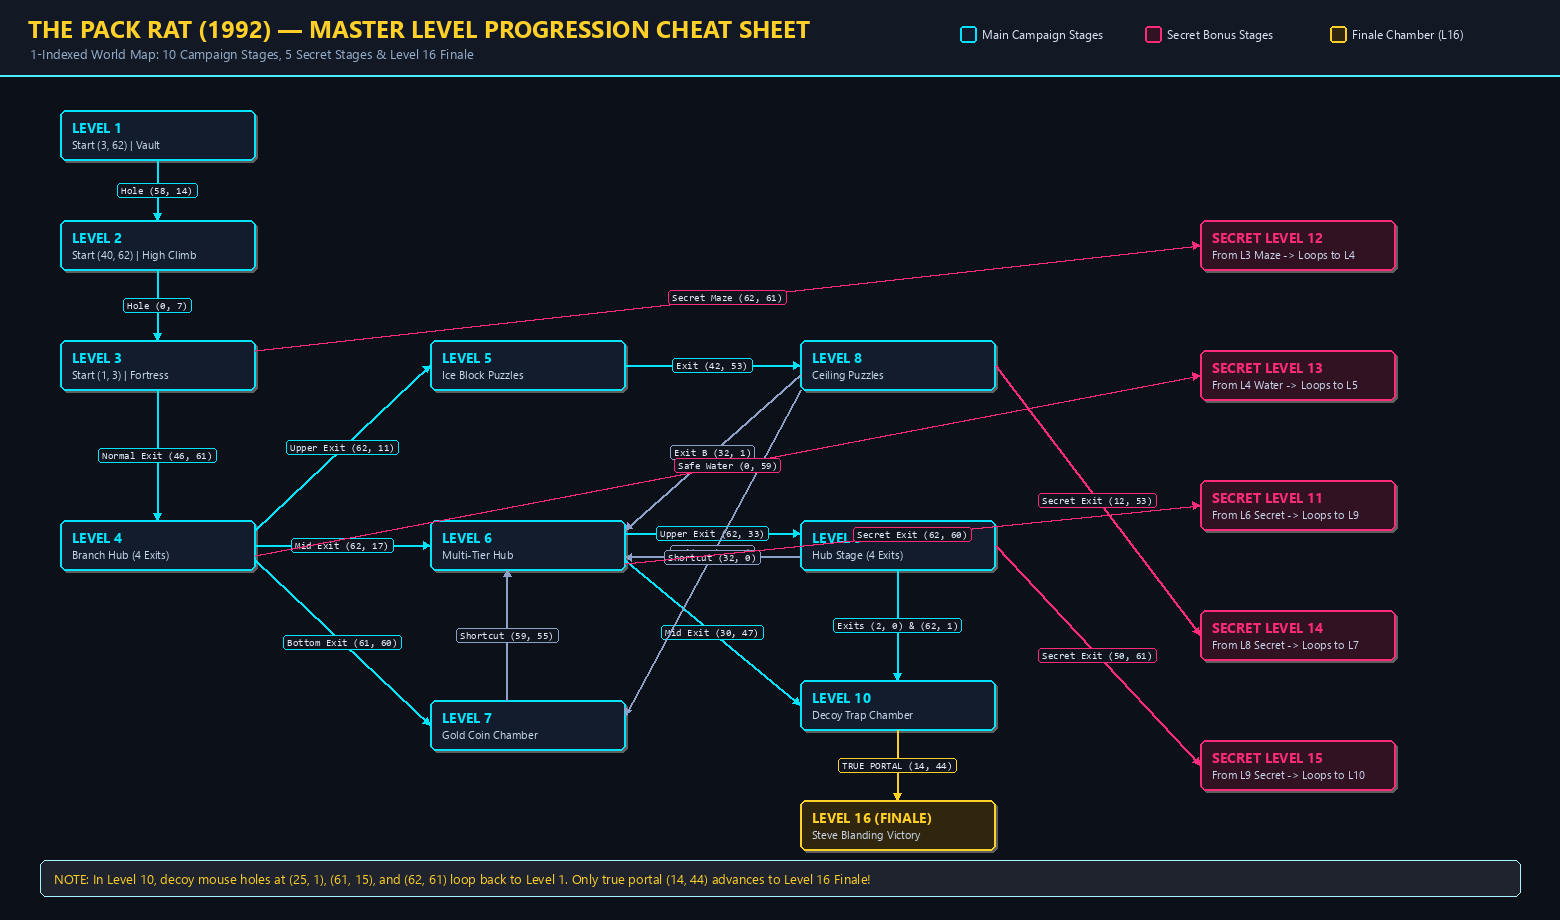
\includegraphics[width=0.76\linewidth,height=2.15in,keepaspectratio]{progression_map.png}%
    }
    \vspace{-3pt}
    \captionof{figure}{\small The Complete 16-Level Progression Network (1-Indexed)}
\end{center}

\vspace{-0.5em}

\subsection{Progression Architecture}
\begin{enumerate}[leftmargin=1.5em,noitemsep]
    \item \textbf{The Spine (Levels 1 $\rightarrow$ 2 $\rightarrow$ 3 $\rightarrow$ 4)}: Every playthrough begins in Level 1 and advances linearly through Level 4.
    \item \textbf{The Level 4 Crossroad}: Level 4 is the grand crossroads of the game. Depending on which mouse hole you enter, you can warp directly to Level 5 (Upper Exit), Level 6 (Middle Exit), Level 7 (Lower Exit), or the secret safe-water tunnel to Level 13!
    \item \textbf{The Convergence on Level 10}: All paths eventually funnel into Level 10 (The Electrical Machine Chamber).
    \item \textbf{The Decoy Danger in Level 10}: In Level 10, three mouse holes are \textbf{decoys} that punish the player by resetting them back to Level 1! Only the hidden high-voltage portal in the central generator room grants access to the \textbf{Level 16 Finale}.
\end{enumerate}

\newpage

\section{The 4 Major Secrets \& Illusionary Passages}
Every secret location below has been verified against the original 1992 DOS real-mode binary data. Clear side-by-side cards provide immediate visual reference alongside step-by-step navigation.

% --- SECRET 1 CARD ---
\begin{secretcard}[cobalt]{SECRET 1: LEVEL 1 — THE SUBTERRANEAN CHEESE VAULT}
\begin{minipage}[c]{0.48\linewidth}
    \centering
    \fboxsep=0pt\fboxrule=0.8pt\fcolorbox{borderline}{white}{%
        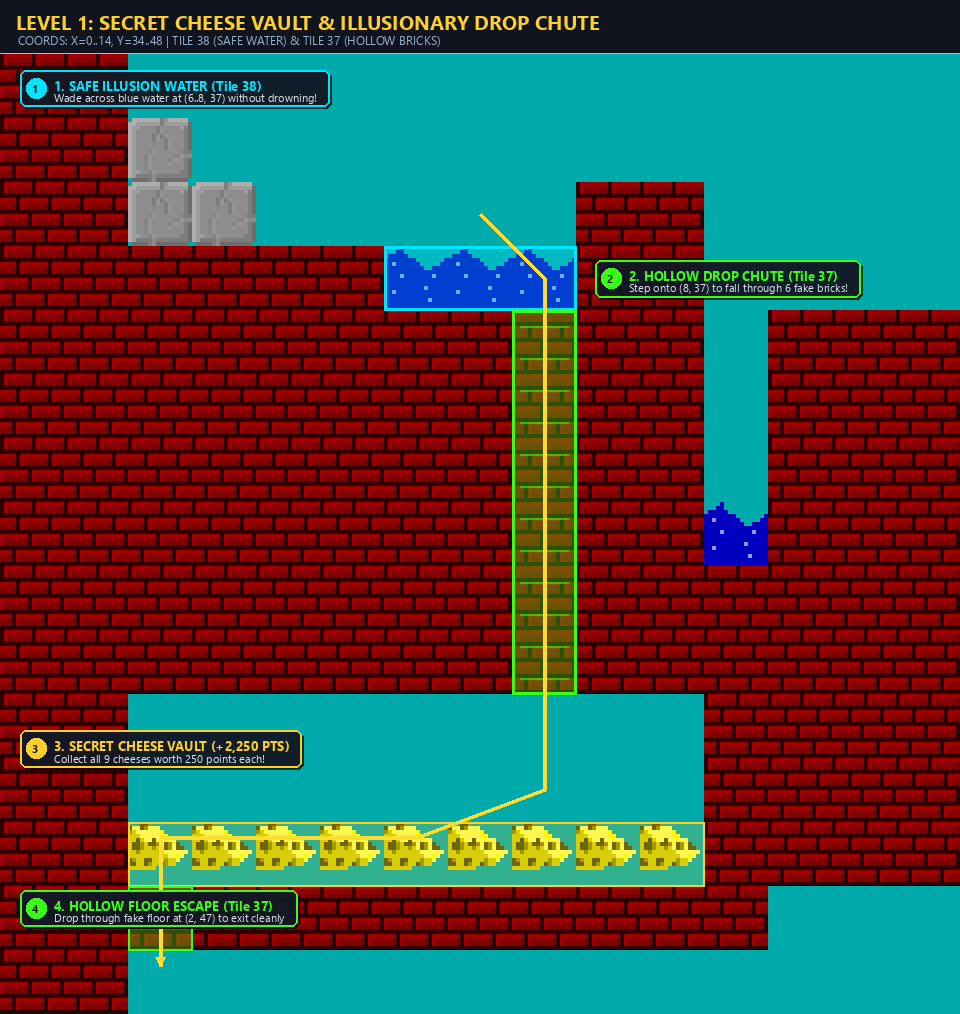
\includegraphics[width=\linewidth,height=1.85in,keepaspectratio]{level1_cheese_vault.png}%
    }
    \vspace{2pt}
    \captionof{figure}{\scriptsize\textbf{Fig 3.1:} Safe Water Trench \& Hollow Brick Chute}
\end{minipage}\hfill
\begin{minipage}[c]{0.49\linewidth}
    {\small\textcolor{teal}{\textbf{Environment:} Living Room Floor \quad\textbullet\quad \textbf{Destination:} Secret Vault (+1,500 pts)}}\\[4pt]
    \renewcommand{\arraystretch}{1.18}
    \scriptsize
    \begin{tabularx}{\linewidth}{@{}l X@{}}
    \textbf{Landmark:} & Begin at spawn on the bottom-left brick floor. Climb staggered ledges along the left wall to the upper reservoir. \\
    \textbf{The Illusion:} & A blue water pool sits at the upper ledge. Unlike normal deep water, this pool is \textbf{illusionary water} and will not drown you! \\
    \textbf{The Route:} & Step into the water pool $\rightarrow$ walk directly through the solid brick pillar on the right (hollow chute) $\rightarrow$ drop down into vault. \\
    \textbf{Reward:} & Collect 5 cheese wedges and gold coins worth over 1,500 bonus points. \\
    \textbf{Escape:} & Step onto the floor tile at bottom-left of the vault. It is a one-way false floor dropping you back to start. \\
    \end{tabularx}
\end{minipage}
\end{secretcard}

% --- SECRET 2 CARD ---
\begin{secretcard}[teal]{SECRET 2: LEVEL 3 — THE 118-TILE SOLID BRICK FORTRESS MAZE}
\begin{minipage}[c]{0.48\linewidth}
    \centering
    \fboxsep=0pt\fboxrule=0.8pt\fcolorbox{borderline}{white}{%
        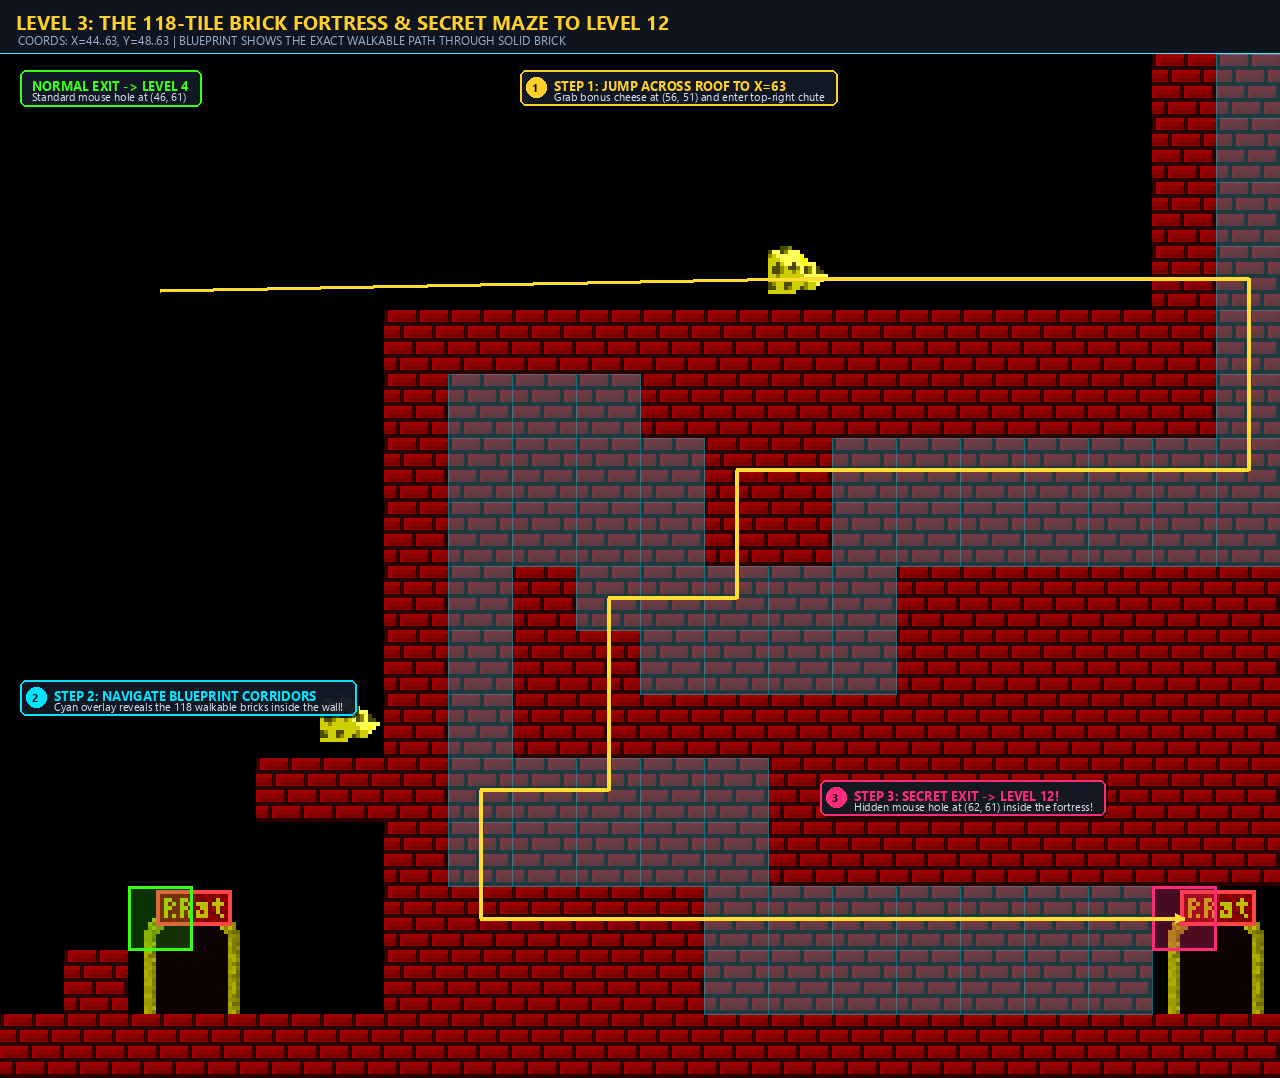
\includegraphics[width=\linewidth,height=1.85in,keepaspectratio]{level3_secret_fortress.png}%
    }
    \vspace{2pt}
    \captionof{figure}{\scriptsize\textbf{Fig 3.2:} The 118-Tile Hollow Brick S-Curve Passage}
\end{minipage}\hfill
\begin{minipage}[c]{0.49\linewidth}
    {\small\textcolor{cobalt}{\textbf{Environment:} Brick Basement \quad\textbullet\quad \textbf{Destination:} Warp to Secret Level 12}}\\[4pt]
    \renewcommand{\arraystretch}{1.18}
    \scriptsize
    \begin{tabularx}{\linewidth}{@{}l X@{}}
    \textbf{Landmark:} & Proceed across Level 3 to the far bottom-right corner. You will encounter a massive, towering wall of solid red brick. \\
    \textbf{The Illusion:} & In reality, an astonishing \textbf{118 brick tiles} in this fortress are completely hollow and permeable! \\
    \textbf{The Route:} & Walk straight into the brick wall along the floor line. Follow the highlighted cyan path: ascend the interior hidden stairway, weave rightward past the structural column, and descend into the sanctum. \\
    \textbf{Reward:} & Hidden mouse hole warps directly into \textbf{Secret Bonus Level 12 (Crystal Caves)}! \\
    \end{tabularx}
\end{minipage}
\end{secretcard}

\newpage

% --- SECRET 3 CARD ---
\begin{secretcard}[cobalt]{SECRET 3: LEVEL 4 — THE SAFE ILLUSIONARY WATER CHANNEL}
\begin{minipage}[c]{0.48\linewidth}
    \centering
    \fboxsep=0pt\fboxrule=0.8pt\fcolorbox{borderline}{white}{%
        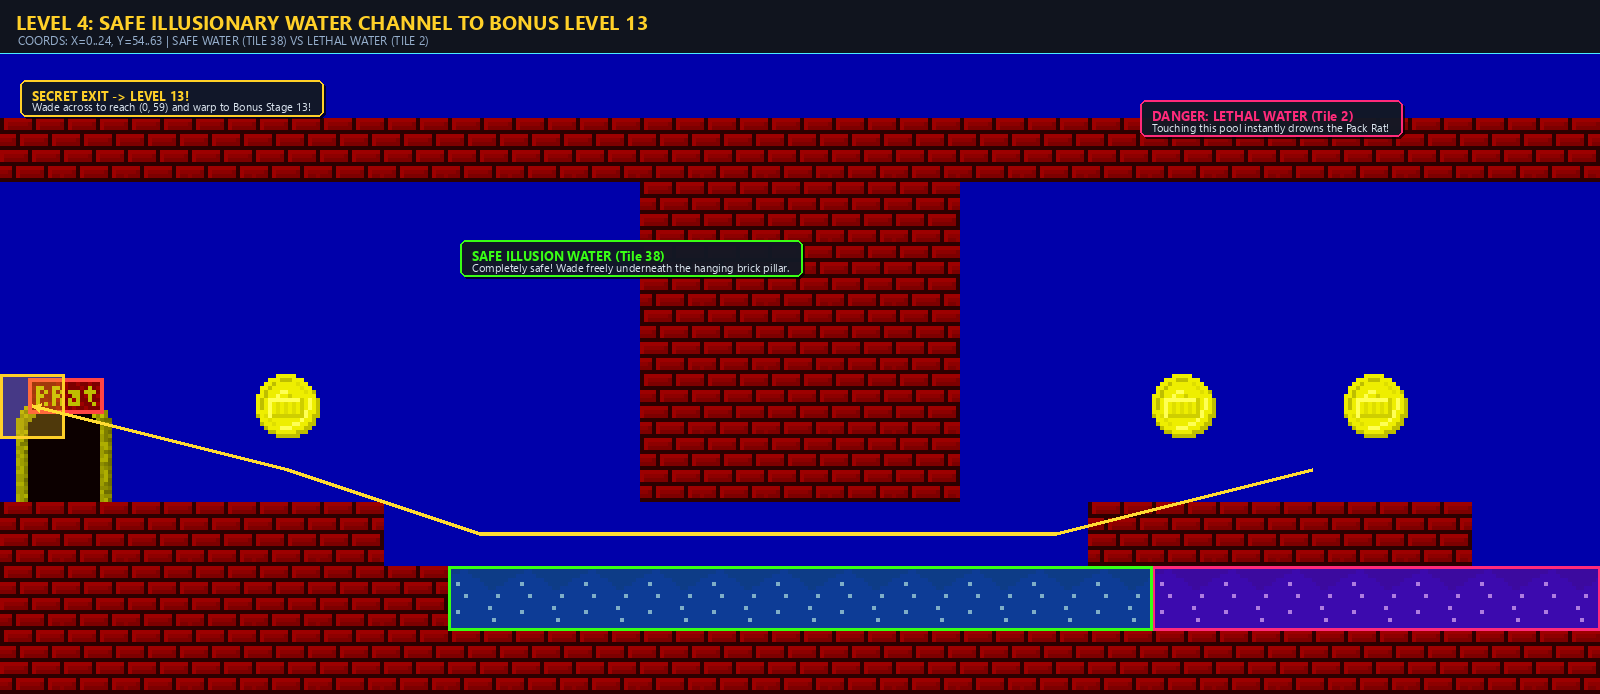
\includegraphics[width=\linewidth,height=1.85in,keepaspectratio]{level4_mousetrap_gauntlet.png}%
    }
    \vspace{2pt}
    \captionof{figure}{\scriptsize\textbf{Fig 3.3:} Safe Shallow Trench vs Lethal Deep Water}
\end{minipage}\hfill
\begin{minipage}[c]{0.49\linewidth}
    {\small\textcolor{teal}{\textbf{Environment:} Flooded Foundations \quad\textbullet\quad \textbf{Destination:} Warp to Secret Level 13}}\\[4pt]
    \renewcommand{\arraystretch}{1.18}
    \scriptsize
    \begin{tabularx}{\linewidth}{@{}l X@{}}
    \textbf{Landmark:} & Drop down to the flooded basement floor in the bottom-left quadrant of Level 4. \\
    \textbf{The Illusion:} & The first 11 water tiles extending rightward from the left wall are \textbf{illusionary shallow water}. The Pack Rat wades freely without taking damage! \\
    \textbf{The Danger:} & To the right of the safe zone lies true deep water. Touching the deep water causes instant drowning death. \\
    \textbf{The Route:} & Wade leftward through the safe trench to the far left wall. Enter the mouse hole nestled against the rock face. \\
    \textbf{Reward:} & Warps directly to \textbf{Secret Bonus Level 13 (Sunken Cellar)}. \\
    \end{tabularx}
\end{minipage}
\end{secretcard}

% --- SECRET 4 CARD ---
\begin{secretcard}[crimson]{SECRET 4: LEVEL 10 — DECOY PITFALL TRAP vs. TRUE FINALE PORTAL}
\begin{minipage}[c]{0.48\linewidth}
    \centering
    \fboxsep=0pt\fboxrule=0.8pt\fcolorbox{borderline}{white}{%
        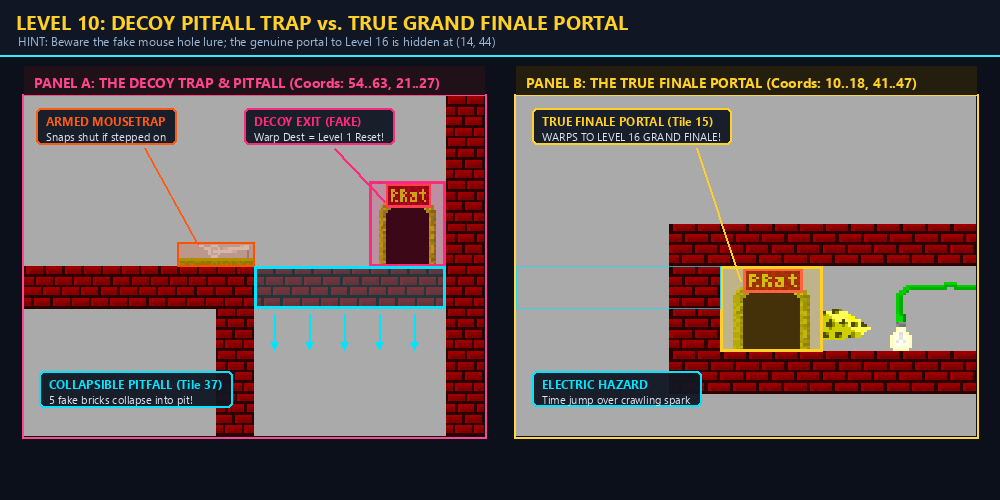
\includegraphics[width=\linewidth,height=1.85in,keepaspectratio]{level10_decoy_trap.png}%
    }
    \vspace{2pt}
    \captionof{figure}{\scriptsize\textbf{Fig 3.4:} Decoy Pitfall Trap (Panel A) vs True Finale Portal (Panel B)}
\end{minipage}\hfill
\begin{minipage}[c]{0.49\linewidth}
    {\small\textcolor{cobalt}{\textbf{Environment:} High-Voltage Machine \quad\textbullet\quad \textbf{Destination:} True Finale Warp (Level 16)}}\\[4pt]
    \renewcommand{\arraystretch}{1.18}
    \scriptsize
    \begin{tabularx}{\linewidth}{@{}l X@{}}
    \textbf{The Trap:} & In the upper-right chamber sits an enticing mouse hole with a P.Rat sign. \textbf{It is a deadly lure!} An armed mousetrap guards the walkway, and the floor beneath it consists of \textbf{5 collapsible fake bricks} that drop you into the pit! \\
    \textbf{Penalty:} & Entering the decoy hole resets the player back to Level 1! \\
    \textbf{True Route:} & Head down to the central generator chamber (coords: 10..18, 41..47). Time your jump over the slow-crawling spark on the green wire. \\
    \textbf{Reward:} & Enter the genuine mouse hole behind the generator coils to warp to the \textbf{Level 16 Grand Finale}! \\
    \end{tabularx}
\end{minipage}
\end{secretcard}

\newpage

\section{Master 16-Stage Directory \& Complete Walkthrough}

\begin{table}[h!]
\centering
\small
\renewcommand{\arraystretch}{1.10}
\begin{tabularx}{\linewidth}{lllX}
\toprule
\textbf{Stage} & \textbf{Internal} & \textbf{Environment} & \textbf{Primary Route \& Objective} \\
\midrule
\textbf{Level 1} & Level 0 & Living Room Floor & Jump rightward across floorboards; avoid bottom pit. Enter mouse hole on right wall. Access Cheese Vault via top-left illusionary pool. \\
\textbf{Level 2} & Level 1 & Pantry \& Cupboards & Climb climbing spools upward. Push sliding ice blocks to create stairs. Exit is at far bottom-left. \\
\textbf{Level 3} & Level 2 & Brick Basement & Standard exit is at bottom-middle. Navigate the 118-tile hollow brick fortress on the bottom-right to reach Secret Level 12. \\
\textbf{Level 4} & Level 3 & Flooded Foundations & Multi-exit hub: Top-right leads to L5; Mid-right leads to L6; Bottom-right leads to L7. Safe water trench on bottom-left leads to Secret L13. \\
\textbf{Level 5} & Level 4 & Kitchen Countertops & Bounce on rubber bands across stove burners. Exit hole is at lower-middle right. Leads directly to Level 8. \\
\textbf{Level 6} & Level 5 & Dining Hall \& Ledges & Patrol rats on long tables. Upper-right exit leads to Level 9; mid-left exit drops to Level 10; secret exit on far right leads to Secret Level 11. \\
\textbf{Level 7} & Level 6 & Storage Closet & Push thread spools down ramps to crush gaps. Mouse hole at upper-right connects back to Level 6. \\
\textbf{Level 8} & Level 7 & Attic Rafters & High-altitude jumps across hanging beams. Left chimney exit leads to Level 7; right rafter exit loops to Level 6; secret chute leads to Secret L14. \\
\textbf{Level 9} & Level 8 & Fireplace Gauntlet & Dodge vertical embers and soot falls. Upper chimney exit connects directly to Level 10. Far right chimney leads to Secret Level 15. \\
\textbf{Level 10} & Level 9 & High-Voltage Machine & Avoid decoy hole on upper right! Enter the electric generator room on middle-left to activate the True Portal to Level 16. \\
\midrule
\textbf{Level 11} & Level 10 & Secret Sewer Pipes & Secret bonus level from Level 6. High-speed pipe transport network; loops cleanly back to Level 9. \\
\textbf{Level 12} & Level 11 & Secret Crystal Caves & Secret bonus level from Level 3. Abundant cheese clusters; loops back into Level 6. \\
\textbf{Level 13} & Level 12 & Secret Sunken Cellar & Secret bonus level from Level 4 safe water. Low-gravity water jumps; loops back into Level 5. \\
\textbf{Level 14} & Level 13 & Secret Attic Vault & Secret bonus level from Level 8. Massive coin cache; loops back into Level 7. \\
\textbf{Level 15} & Level 14 & Secret Clock Tower & Secret bonus level from Level 9. Swinging pendulum spools; loops back into Level 10. \\
\midrule
\textbf{Level 16} & Level 15 & The Grand Finale & The supreme challenge! Timed high-voltage spark gauntlet, precision block slides, and the final Golden Trophy Room! \\
\bottomrule
\end{tabularx}
\caption{The Complete 16-Stage World Directory}
\end{table}

\vspace{-0.3em}

\section{Essential Survival Mechanics}

\begin{enumerate}[leftmargin=1.5em,itemsep=2pt]
    \item \textbf{Thread Spools (Push \& Climb)}:
    \begin{itemize}[noitemsep]
        \item Spools act as solid platforms. Pushing against one causes it to roll smoothly across flat ground until it hits a wall or ledge.
        \item When touching a vertical column of spools, hold the \textbf{Up} key to climb upward like a ladder, or press \textbf{Down} to descend safely one spool at a time.
    \end{itemize}

    \item \textbf{Rubber Bands (The Trampoline Effect)}:
    \begin{itemize}[noitemsep]
        \item Landing on a red rubber band tile bounces the Pack Rat upward automatically.
        \item \textbf{Pro Tip}: Holding down the \textbf{Jump} button as you strike the rubber band delivers a \emph{Super Trampoline Bounce}, propelling you nearly twice as high!
        \item You can jump upward through rubber bands from underneath without hitting your head.
    \end{itemize}

    \item \textbf{Ice Blocks (The 3-Push Mechanic)}:
    \begin{itemize}[noitemsep]
        \item Transparent ice blocks require \textbf{three distinct push hits} while holding the Push button to slide horizontally.
        \item Crouching directly on top of an ice block and pressing down three times will dislodge it below you, allowing you to drop into sealed lower chambers.
    \end{itemize}

    \item \textbf{The Emergency Suicide Key (\texttt{K})}:
    \begin{itemize}[noitemsep]
        \item If you accidentally box yourself in with heavy sliding blocks or get wedged behind one-way drops, press the \textbf{K} key to restart the current room without losing your overall game progress.
    \end{itemize}

    \item \textbf{Testing \& Exploration God Mode (\texttt{I})}:
    \begin{itemize}[noitemsep]
        \item Press the \textbf{I} key (or click the \textbf{GOD} button on the top arcade header) to toggle \textbf{Invincibility \& Unlimited Lives}.
        \item In God Mode, the Pack Rat is completely immune to mousetraps, live electrical currents, deep water pools, and enemy rat patrols, allowing frictionless level inspection and testing.
    \end{itemize}
\end{enumerate}

\vspace{0.3em}
\begin{center}
    \rule{0.6\linewidth}{0.8pt}\\[3pt]
    \textsc{\small Pack Rat Preservation Project \quad\textbullet\quad Authentic 1992 DOS Reconstruction \quad\textbullet\quad Happy Hunting!}
\end{center}

\end{document}
